\documentclass{article}

% to compile a camera-ready version, add the [final] option, e.g.:
\usepackage[final]{neurips_2021}

\usepackage[utf8]{inputenc} % allow utf-8 input
\usepackage[T1]{fontenc}    % use 8-bit T1 fonts
\usepackage{hyperref}       % hyperlinks
\usepackage{url}            % simple URL typesetting
\usepackage{booktabs}       % professional-quality tables
\usepackage{amsfonts}       % blackboard math symbols
\usepackage{nicefrac}       % compact symbols for 1/2, etc.
\usepackage{microtype}      % microtypography
\usepackage{xcolor}         % colors

\usepackage{listings}
\definecolor{dkgreen}{rgb}{0,0.6,0}
\definecolor{gray}{rgb}{0.5,0.5,0.5}
\definecolor{mauve}{rgb}{0.58,0,0.82}
\lstset{frame=tb,
  language=python,
  aboveskip=3mm,
  belowskip=3mm,
  showstringspaces=false,
  columns=flexible,
  basicstyle={\small\ttfamily},
  numbers=none,
  numberstyle=\tiny\color{gray},
  keywordstyle=\color{blue},
  commentstyle=\color{dkgreen},
  stringstyle=\color{mauve},
  breaklines=true,
  breakatwhitespace=true,
  tabsize=3
}
\usepackage{graphicx}

\title{
NLP Classification Models for the 20 Newsgroups Dataset, and Exploratory Data Analysis for a Curriculum-Alignment NLP Model  \\
}

\author{%
  Mathew ~Bushuru \\
  81262800\\
  ELEC 400M Final Report\\
  University of British Columbia\\ 
  \texttt{mathewbw@student.ubc.ca} \\
  December 16,2022\\
}

\begin{document}

\maketitle

\begin{abstract}
  The act of teaching and learning is almost as old as humanity itself, but technological advancement in the past few decades has drastically altered the way it is done. This project lays the foundation for a machine-learning model to be used to create a curriculum alignment recommendation tool. This model will use Natural Language Processing (NLP) to predict the content items best aligned to a given topic when creating a curriculum from online open-source educational materials. The scope of this project is to do data preprocessing and exploratory data analysis for this model. In addition to this, a related machine learning project is fully implemented using similar data of lower complexity. We build two models: a naive Bayes classifier and a Support Vector Machine (SVM) model. The goal of these models is to group raw text data of several newsgroups posts into different categories describing what the post is about. We then use cross-validation to improve the performance of these models. The goal of the curriculum-alignment model is similar; to use the raw text data of content items to align them to different topic trees. Therefore, the lessons learnt from these two newsgroups models will be instrumental in implementing the more complex model as part of a Kaggle competition due on March 14,2023.
\end{abstract}

\section{Introduction and Problem Setup}

\subsection{Background}
The value of education cannot be understated. Article 26 of the United Nations Universal Declaration of Human Rights gives every human a right to education. Technology has played a pivotal role in transforming the education industry over the past few years. The COVID-19 pandemic increased the role of technology in education even further with remote education and internet access becoming a necessity. However, this shift exposed the digital divide gap among low-income societies around the world. A study by GSMA on the state of internet connectivity [16] found that 40 percent of the world's population does not have access to the internet.

In 2019, I tried to tackle this problem. Together with two of my peers, we registered to participate in a social-venture-focused hackathon. The idea was to identify online open-source educational content and load it on a Raspberry Pi running on a headless Linux operating system that had been modified to work as an internet server. This content with preloaded educational content would then be used in schools without internet access. We also built software to enable users to access the different learning resources on  the content server. One challenge we faced was it was really time-consuming and resource-intensive to align the online educational content designed for different educational systems to the Kenyan education system. 

\subsection{Learning Equality Kaggle Competition - Curriculum Recommendations}
After working on this problem for a few months, we came across a non-profit organization called Learning Equality working on the same problem but on a global scale. Their platform, Kolibri, organizes open-source content for each country separately. However, each country has its own educational structures and objectives making it difficult for educators to use a specific country's educational content from different countries. To solve this challenge, Learning Equality announced a Kaggle competition. 

\subsection{Machine learning Problem}

\subsubsection{Curriculum-alignment machine learning problem}
The goal is to use machine learning techniques to automate the curriculum alignment procedure. When curating content for a specific topic within a specific country's curriculum, the user is presented with relevant content items from the Kolibri Library [1]. We create a model using a dataset of K-12 educational materials which can predict which content items are best aligned to a given topic. An example of the model output is shown below:

\begin{lstlisting}
topic_id,content_ids
t_00004da3a1b2,c_1108dd0c7a5d c_376c5a8eb028 c_5bc0e1e2cba0 c_76231f9d0b5e
t_00068291e9a4,c_639ea2ef9c95 c_89ce9367be10 c_ac1672cdcd2c c_ebb7fdf10a7e
t_00069b63a70a,c_11a1dc0bfb99
...
\end{lstlisting}

For each \texttt{text\_id}, the model predicts a space-delimited list of recommended \texttt{content\_ids} for that topic. The timeline for this Kaggle competition is:

 \begin{itemize}
     \item December 15, 2022 - Start Date.
     \item March 7, 2023 - Entry Deadline. You must accept the competition rules before this date in order to compete.
     \item March 7, 2023 - Team Merger Deadline. This is the last day participants may join or merge team
     \item March 14, 2023 - Final Submission Deadline.
 \end{itemize}

\subsubsection{20 newsgroups data machine learning problem}

For this project, we will work on a  supervised learning problem using the 20 newsgroups data. The machine learning task is to build an NLP multi-classification model. The data consists of 18000 newsgroup posts evenly split among 20 topics. The data we build with this model will allow us to predict a particular topic when presented with a string. An example is shown below:

\begin{lstlisting}
def predict(string,X_train = newsgroups_train, model = nb_pipeline_model):
  prediction = model.predict([string])
  return X_train.target_names[prediction[0]]
predict("Canada")
> rec.sport.hockey
\end{lstlisting}

\subsection{Relevant applications}

Applications of NLP classifiers include 
\begin{itemize}
    \item Spam detection in emails
    \item Sentiment analysis in social media 
    \item Topic detection in chatbots
\end{itemize}

\subsection{Data set}

\subsubsection{20 newsgroups dataset} 

This dataset was collected by Ken Lang [6]. It is a collection of about 18000 newsgroups posts on 20 topics split into a training dataset and a testing dataset. We build a text classification model using this data.

\subsubsection{Curriculum alignment dataset} 
This dataset contains the correlations between the specific content items and topics from the K-12 curriculum. The data is organized according to topics. The data is contained in three different files: \texttt{topic.csv},  \texttt{correlations.csv}, and  \texttt{content.csv}. For this project, we will preprocess this data to be ready for NLP classification [1].

\section{Data Analysis}

\subsection{Exploratory Data Analysis on curriculum-alignment dataset}
Next, we explore the different files and fields in the dataset referencing [1]

\subsubsection{\texttt{correlations.csv}}
This data contains a row of unique \texttt{topic\_ids} with all the corresponding \texttt{content\_ids}. Not all \texttt{topic\_ids} have content and these are represented with \texttt{NaN}. A \texttt{topic\_id} can have one or more \texttt{content\_ids}.
\begin{lstlisting}
     topic_id              content_ids
  0  t_00004da3a1b2        c_1108dd0c7a5d c_376c5a8eb028 c_5bc0e1e2cba0 c...
  1  t_00068291e9a4	     c_639ea2ef9c95 c_89ce9367be10 c_ac1672cdcd2c c...
  2  t_00069b63a70a	     c_11a1dc0bfb99
\end{lstlisting}

\subsubsection{\texttt{content.csv}}
Contains a row for each content item in the dataset. Some content items may not be correlated with any topic. [1]

\begin{itemize}
    
\item  \texttt{id} - A unique identifier for this content item.

\item  \texttt{title} - Title text for this content item.

\item  \texttt{description} - Description text. May be empty.

\item  \texttt{language} - Language code representing the language of this content item.

\item  \texttt{kind} - Describes what format of content this item represents, as one of:

\begin{itemize}
    \item \texttt{document} (text is extracted from a PDF or EPUB file)
    \item \texttt{document} (text is extracted from a PDF or EPUB file)

    \item \texttt{video} (text is extracted from the subtitle file, if available)

     \item \texttt{exercise} (text is extracted from questions/answers)

    \item \texttt{audio} (no text)

    \item \texttt{html5} (text is extracted from HTML source)
    
\end{itemize}

\item  \texttt{text} - Extracted text content, if available and if licensing permitted (around half of content items have text content).

\item  \texttt{copyright\_holder} - If text was extracted from the content, indicates the owner of the copyright for that content. Blank for all test set items.

\item  \texttt{license} - If text was extracted from the content, the license under which that content was made available. Blank for all test set items.

\end{itemize}

\subsubsection{\texttt{topic.csv}} 

This contains each topic in the dataset[1].

\begin{itemize}
    
\item  \texttt{id} - A unique identifier for this topic.

\item  \texttt{title} - Title text for this topic.

\item  \texttt{description} - Description text. May be empty.

\item  \texttt{language} - Language code for the topic.

\item  \texttt{category} - Describes the origin of the topic:

\begin{itemize}
    \item \texttt{source} (structure was given by original content creator (e.g. the topic tree as imported from Khan Academy))
    
    \item \texttt{aligned} (Structure is from a national curriculum or other target taxonomy, with content aligned from multiple sources)

    \item \texttt{supplemental} (This is a channel that has to some extent been aligned, with without the same level of granularity or fidelity as an aligned channel.) 
    
\end{itemize}

\item  \texttt{channel} - The topic tree the topic is part of

\item  \texttt{has\_content} - Whether there are content items correlated with this topic. Most content is correlated with leaf topics, but some non-leaf topics also have content correlations

\item  \texttt{parent} - The id of the topic that contains this topic, if any. This field if empty if the topic is the root node for its channel

\end{itemize} 

\subsubsection{Missing values}

We then investigate the sparsity of our dataset. The figure 1 shows the frequency of occurrences in a random sample of our \texttt{content\_data}

\begin{figure}[htp]
    \centering
    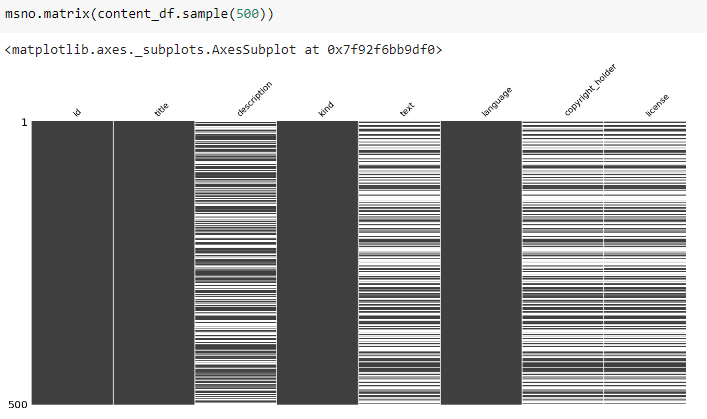
\includegraphics[width=12cm]{content_sparsity.png}
    \caption{Content Sparsity Matrix}
    \label{fig:galaxy}
\end{figure}

The description, text content, copyright holder and license  fields only occur about 50 percent of the time in our content data. The corresponding sparsity matrix for topic data is shown on figure 2. 

The model we build will have to find the relationship between the occurrences of words in the textual data input  e.g content title, content text, etc. and the occurrences of similar words in the textual output fields which will act as y

\begin{figure}[htp]
    \centering
    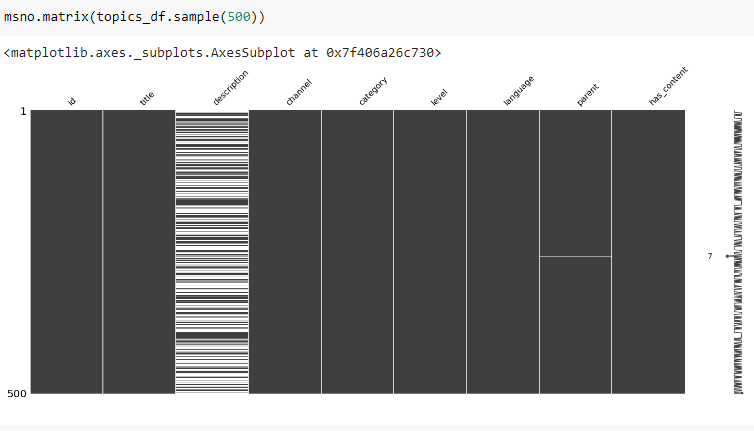
\includegraphics[width=14cm]{topic_sparsity.png}
    \caption{Topic sparsity matrix}
    \label{fig:galaxy}
\end{figure} 

\subsubsection{Value Counts} 

We then investigate the occurrences of the different classes in the dataset. A bar plot of the occurrences of languages in the content data is shown on figure 3.

\begin{figure}[htp]
    \centering
    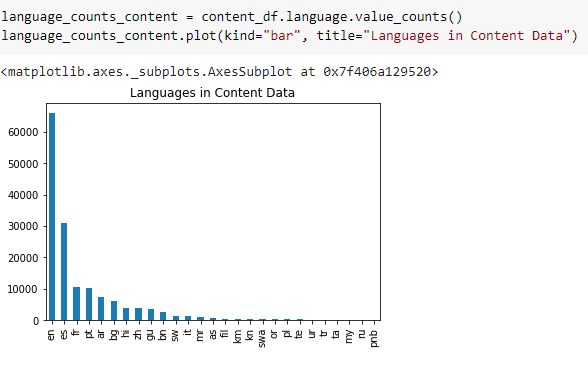
\includegraphics[width=14cm]{language_figure_counts.png}
    \caption{Occurrences of language types in content data}
    \label{fig:galaxy}
\end{figure}  

English is the predominant language in the data. This means English-based NLP models are a viable option for this model. However, for better performance, we use a multi-language NLP model. The rest of the value counts are in the accompanying Jupyter notebook.

\subsection{Exploratory Data Analysis on 20 newsgroups dataset} 

The dataset contains training data
\begin{equation}
  D =  {(x1,y1),(x2,y2),...,(xn,yn)}
\end{equation}
which trains a model to give us the target 
 \begin{equation}
y
\end{equation}
which can be one of K different values. If K=2 such as in positive or negative sentiment analysis, it is referred to as binary classification.
\begin{equation}
Y = {y_1,y_2,..,y_k}
\end{equation}

Both the input and output are a sequence of words. We obtained the data from \texttt{sklearn}'s built-in datasets. \texttt{Sklearn} has a loader that enables us to obtain raw text data. Although another loader exists of preprocessed data in form of feature vectors, it was not used. This was for the learning experience and to allow us to have access to custom parameters that we can fine-tune to improve performance.

Each input post in the data consists of: From, Subject, Nntp-Posting-Host, Organization, lines, The rest of the content of the post. An example of one post is shown below

\begin{lstlisting}
From: lerxst@wam.umd.edu (wheres my thing)
Subject: WHAT car is this!?
Nntp-Posting-Host: rac3.wam.umd.edu
Organization: University of Maryland, College Park
Lines: 15

 I was wondering if anyone out there could enlighten me on this car I saw
the other day. It was a 2-door sports car, looked to be from the late 60s/
early 70s. It was called a Bricklin. The doors were really small. In addition,
the front bumper was separate from the rest of the body. This is 
all I know. If anyone can tellme a model name, engine specs, years
of production, where this car is made, history, or whatever info you
have on this funky looking car, please e-mail.

Thanks,
- IL
   ---- brought to you by your neighborhood Lerxst ----
\end{lstlisting} 

All possible  20 labels for the newsgroups posts are shown below:

\begin{lstlisting}
    ['alt.atheism', 'comp.graphics', 'comp.os.ms-windows.misc', 'comp.sys.ibm.pc.hardware', 'comp.sys.mac.hardware', 'comp.windows.x', 'misc.forsale', 'rec.autos', 'rec.motorcycles', 'rec.sport.baseball', 'rec.sport.hockey', 'sci.crypt', 'sci.electronics', 'sci.med', 'sci.space', 'soc.religion.christian', 'talk.politics.guns', 'talk.politics.mideast', 'talk.politics.misc', 'talk.religion.misc']
\end{lstlisting} 

The 20 newsgroups data is not as complex as the curriculum-alignment data. However, they share a common structure where we need to use the occurrences of words in input X to determine the label in output y. Using the newsgroups data, we can come up with NLP classifier models which will be the focus of this final term report. In the next few months, these models will be adapted to work with the curriculum-alignment data

\section{Methodological Approach}

\subsection{Related models and algorithms}

The dimensionality of our data is large and it is linearly proportional to the vocabulary size of the dataset. The most common algorithm used in NLP text classifiers is The Bag of Words. It represents raw text data as a multiset ("bag") of words where the frequency of occurrence of each word is used as a feature vector of training the model [5]. We will use this algorithm in this project.

NLP classifiers can be implemented in a variety of ways but the most popular approaches are using \texttt{naive Bayes classifiers}, \texttt{Support Vector Machines} (SVMs) and Deep Learning. We will be implementing a \texttt{naive Bayes classifier} and an \texttt{SVM} model in this project

\subsection{Data Preprocessing}

However, before we implement the models, we need to transform the textual data into a form that is machine-readable. The input data consists of sequences of words of varying lengths. The first step is to convert the data into d-dimensional numerical vectors using the \texttt{Bag of Words} algorithm 

 we represent all words in the vocabulary of the training set as shown below
\begin{equation}
V = {motoring, mohan,mongoose,atheism ...}
\end{equation}
We then use the \texttt{Term Frequency times Inverse Document Frequency} (TDIDF) vectorizer from \texttt{sklearn} to create the numerical vectors. The resulting data is very sparse and high-dimensional. There are only 157 non-zero vectors out of the huge dataset. This will have a very big impact on the types of models we are able to use. 

\subsection{Naive Bayes NLP Classifier for 20 Newsgroups Data}

There are two types of classification models: generative and disciminative models. Generative models model both input X and output Y, while discriminative models model only output Y given X [11]. A discriminative model would not be suitable for text classification like our problem since the data does not follow a normal distribution. It follows a discrete multinomial distribution

Naive Bayes is a generative classification model. This is because it specifies a hypothetical random process to generate data. Naive Bayes models are usually suitable for high-dimensional data like ours. It uses the Bayes rule shown below
\begin{equation}
arg\:max_{y}\:log\:p\:(y|x) = arg\:max_{y}\:log\:\frac{p\:(x|y)\:p(y)} {p(x)} = arg\:max_{y}\:log\:p\:(x|y)\:p(y)
\end{equation} 

There are several types of naive Bayes models such as Gaussian Naive Bayes and Multinomial Naive Bayes. The difference is in the assumptions they make about data. For this project, the most suitable is Multinomial Naive Bayes which assumes the features are in a multinomial distribution. It describes probabilities of observing counts among a number of categories hence it is perfect for data with count rates like ours[10]. As described above, we preprocess the data to have words represented by their frequency in the raw data.  One disadvantage of naive bayesian classifiers is class conditional independence which impacts the model accuracy for highly correlated data[12]. However, this does not apply to our data because of its high dimensionality. We then build a naive Bayes classifier model. For the hyperparameters, we use the default values and choose an arbitrary value of 0.001 

\section{Results and Data Analysis}

\subsection{Naive Bayes Model Results}

After training the naive Bayes on the \texttt{train\_data}, we get an \texttt{accuracy} of 0.835 and an \texttt{f1\_score} of 0.829. The classification report is shown in figure 4 

\begin{figure}[htp]
    \centering
    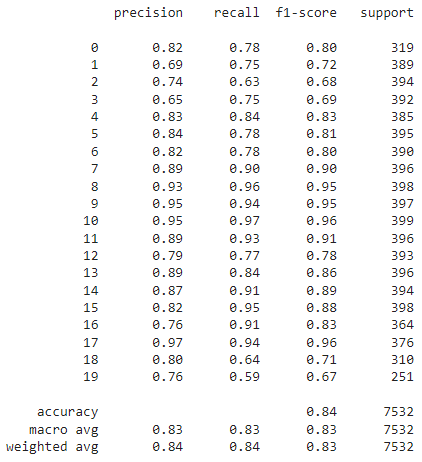
\includegraphics[width=8cm]{nb_csf_report.png}
    \caption{Naive Bayes Model's Classification Report}
    \label{fig:galaxy}
\end{figure}  

\subsection{Hyperparameter Tuning and Cross Validation for Naive Bayes Model} 

To perform cross validation, we shuffle the dataset randomly and split the dataset into k groups. Here, we will take k=5, for 5 fold cross validation. For each group, we hold out one as the test set and use the remaining for training[11]. I decided to use k-fold cross validation instead of leave-one-out cross validation because it is faster to compute. 

For the hyperparameter tuning, I optimized the value of the alpha parameter. 

Using the \texttt{GridSearchCV} method from \texttt{sklearn} we improve our model's score to 0.9111 and the optimal alpha was found to be 0.01.

\begin{lstlisting}
    grid_search_nb_clf.best_score_ 
    >  0.911171879303898
    grid_search_nb_clf.best_params_
    >  {'alpha': 0.01}
\end{lstlisting} 

\subsection{Alternative Support Vector Machine NLP Classifier Model for 20 Newsgroups Data} 
Support vector machines are suitable for a project like this because they work well with high-dimensional data like ours. This is because they are only affected by points close to the margins. In fact, data that may seem inseparable in lower dimensions might become separable using SVMs after increasing its dimensionality [13]. 

My first approach was to build an SVM model using the \texttt{SVC} method from \texttt{sklearn.svm}. This took a relatively longer training time (~ 4 minutes) on Google Collab. This is because SVC models scale with number of samples  $\mathcal{O}[N^2]$  and since our data has numerous samples (~20k), it requires a lot of computational resources [9] 

A workaround to the intensive support vector machine's computationally intensive calculations is to use the gradient descent algorithm to iteratively find the optimal solution[14]. With  b  as the batch size and  n  as learning rate, we get the following equations for a stochastic gradient descent algorithm:

\begin{equation}
    {\theta}_{t+1} \: = {\theta}_{t}\: - ng\:{\theta}_{t}
\end{equation}

with 
\begin{equation}
g({\theta}_{t}\:) \: = \frac{1}{b}\: \sum_{i\subset}\: \Delta_{\theta} \: l\: (x_{i},\:\theta_{t})
\end{equation} 

Stochastic Gradient Descent model on \texttt{sklearn} implements linear classifiers such as SVM and logistic regression with stochastic gradient descent. The \texttt{sklearn} model works best with sparse data. As we saw above, the data we're using is sparse making this a suitable model. We choose \texttt{hinge} loss so that the model implements a linear SVM. We use \texttt{l2} for the regularization term which is standard for linear SVM models. We pick an arbitrary value of alpha (0.0001) for the first training. Training this model on our vectorized data is considerably faster than the previous SVC model ( ~2 seconds compared to ~ 4 minutes in the same runtime session) 

After training the SVM model on the \texttt{train\_data}, we get an \texttt{accuracy} of 0.824 and an \texttt{f1\_score} of 0.810. The classification report is shown in figure 5.

\begin{figure}[htp]
    \centering
    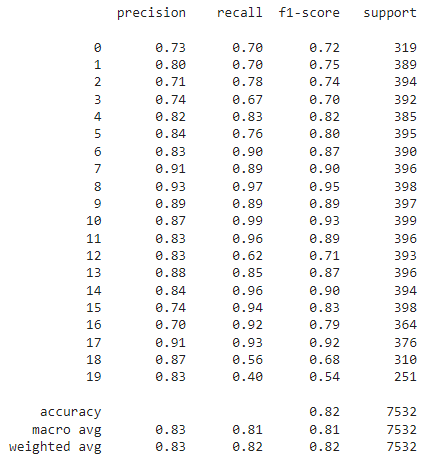
\includegraphics[width=8cm]{svm_csf_report.png}
    \caption{SVM Model's Classification Report}
    \label{fig:galaxy}
\end{figure} 

We pass the SVM model through a cross-validation and hyperparameter tuning similar to the naive classifier model. Using the \texttt{GridSearchCV} method from \texttt{sklearn}  improved our model's score to 0.889 and the optimal alpha was found to be 0.01 

\begin{lstlisting}
    grid_search_svm_clf.best_score_
    >  0.8889869046237614
    grid_search_svm_clf.best_params_
    >  {'alpha': 0.001}
\end{lstlisting} 

The bar plot in figure 6 shows the effect of tuning the alpha parameters for both the SVM model and the naive Bayes model, and performing a 5-fold cross validation.
\begin{figure}[htp]
    \centering
    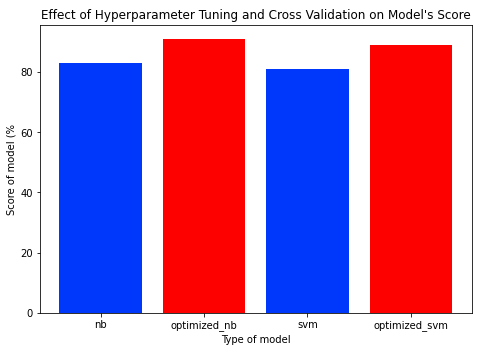
\includegraphics[width=12cm]{bar.png}
    \caption{Effect of hyperparameter tuning and 5 fold cross validation}
    \label{fig:galaxy}
\end{figure} 
 
\section{Discussion}

Using the \texttt{predict()} method, we can create a pipeline that receives a string of text and returns a category that has the highest probability of being correlated to the provided string. An example is shown below.
\begin{lstlisting}
def predict(string,X_train = newsgroups_train, model = nb_pipeline_model):
  prediction = model.predict([string])
  return X_train.target_names[prediction[0]]
predict("Canada")
> rec.sport.hockey
\end{lstlisting}

Keeping in mind that we trained our model on data with only 20 categories (that did not include countries), it is impressive that a simple probabilistic model based on the frequency of words can create an association between Canada and hockey. 

\subsection{Future directions}
Some options that could be used to improve these two models include: 
\begin{itemize}
    \item Filtering common words such as articles 'a', 'an' and 'the'. When we looked at the \texttt{top\_5\_features} function, both 'to' and 'for' were in each of the top 5 so filtering them would improve performance.
    \item Further preprocessing the data to only keep the word roots. For example, mapping both 'happily' and 'happiness' to happy [7]
\end{itemize}

\subsection{Adapt NLP models to curriculum-alignment data} 
As a starting point, the next step would be to filter out the input \texttt{X\_data} that has \texttt{text\_content} in the curriculum recommendation data. The text content e.g. the entire text of a textbook would be similar to the input post content in the 20 newsgroups data. For the y-dependent variable, choosing the title text would be similar to the categories in the newsgroups. The reasoning for this is most educational content contains the name of the topic in the title e.g. "Grade 11 Biology" and can thus be a stand-in for the expected output. 

\subsection{Challenges} 
One of the biggest challenges in this project was frequently hitting the maximum compute units limit on Google Collab. This occurred mostly when preprocessing the curriculum data. A possible solution going forward is to explore deep learning models for natural language processing that are able to use GPUs for computation. 

\subsection{Code}
Code for this project can be found at: https://github.com/mathewbushuru/ml-curriculum-recommender 

This contains:
\begin{itemize}
    \item This report in PDF
    \item Full Jupyter Notebook with all the relevant explanations
    \item Jupyter Notebook Consisting of just the relevant code
    \item Latex files for this project
\end{itemize}

\section*{References}
\medskip

{
\small

[1] References "Learning Equality - Curriculum Recommendations." (2022). Retrieved from https://kaggle.com/competitions/learning-equality-curriculum-recommendations

[2] References "Using Missingno to Diagnose Data Sparsity." (2022). Retrieved from https://www.kaggle.com/code/residentmario/using-missingno-to-diagnose-data-sparsity 

[3] References "Machine Learning, NLP: Text Classification using scikit-learn, python and NLTK." (2017). Retrieved from https://towardsdatascience.com/machine-learning-nlp-text-classification-using-scikit-learn-python-and-nltk-c52b92a7c73a

[4] References "The 20 newsgroups text dataset" . (2022). Retrieved from https://scikit-learn.org/0.19/datasets/twenty_newsgroups.html 

[5] References "Bag-of-words model". (2022). Retrieved from https://en.wikipedia.org/wiki/Bag-of-words_model 

[6] References "20 Newsgroups"  http://qwone.com/~jason/20Newsgroups/ 

[7] References "Naive Baise Lecture 8 Slides". (2022). Retrieved from https://canvas.cornell.edu/files/2122690/download?download_frd=1 

[8] References "sklearn.linear_model.SGDClassifier". (2022). Retrieved from https://scikit-learn.org/stable/modules/generated/sklearn.linear_model.SGDClassifier.html

[9] References "University of British Columbia's ELEC 400M Class Code Examples - SVM". (2022). Xiaoxiao Li.

[10] References "Python Data Science Handbook". (2016). Jake Vanderplas. O'Reilly Media. 

[11] References "University of British Columbia's ELEC 400M Lecture 6: Model Evaluation and Training". (2022). Xiaoxiao Li.  

[12] References "University of British Columbia's ELEC 400M Lecture 7: Naive Bayesian Classifier". (2022). Xiaoxiao Li.  

[13] References "University of British Columbia's ELEC 400M Lecture 9: Support Vector Machines 2". (2022). Xiaoxiao Li. 

[14] References "University of British Columbia's ELEC 400M Lecture 17: Neural Network Basis". (2022). Xiaoxiao Li.

[15] References "Are Our Children Learning Report". 
 (2020). Retrieved from https://www.humanitarianresponse.info/es/operations/kenya/document/uwezo-2020-are-our-children-learning-status-remote-learning-among-school 

 [16] References "The State of Mobile Internet Connectivity 2022". (2022). Retrieved from https://www.gsma.com/r/somic/
 
}



\end{document}